\documentclass[times, utf8, seminar]{fer}
\usepackage{algorithmic}
\usepackage{algorithm}
\usepackage{booktabs}
\usepackage{listings}
\usepackage{xcolor}
\newcommand\myworries[1]{\textcolor{red}{#1}}
\usepackage{hyperref} 
\usepackage{natbib}
\usepackage{subfig}
\usepackage{color}
\usepackage{placeins}
\usepackage{multirow}

\definecolor{mygreen}{rgb}{0,0.6,0}
\definecolor{mygray}{rgb}{0.5,0.5,0.5}
\definecolor{mymauve}{rgb}{0.58,0,0.82}
\renewcommand\labelitemi{•}

\lstset{ %
  backgroundcolor=\color{white},   % choose the background color
  basicstyle=\footnotesize,        % size of fonts used for the code
  breaklines=true,                 % automatic line breaking only at whitespace
  captionpos=b,                    % sets the caption-position to bottom
  commentstyle=\color{mygreen},    % comment style
  escapeinside={\%*}{*)},          % if you want to add LaTeX within your code
  keywordstyle=\color{blue},       % keyword style
  stringstyle=\color{mymauve},     % string literal style
}
\begin{document}


\title{Međujezično prepoznavanje imenovanih entiteta pomoću wikifikacije}

% TODO: Navedite vaše ime i prezime.
\author{Stipan Mikulić}
\voditelj{dr. sc. Jan Šnajder}

\maketitle

\tableofcontents

\chapter{Uvod}
U današnje vrijeme svjedočimo stalni eksponencijali porast svih vrsta podataka, naročito teksta. Zbog tog naglog porasta podataka ljudi više nisu u mogućnosti obraditi te podatke da bi prepoznali bitne i korisne informacije. Riješenje problema krije se u računalnoj obradi podataka. 
Ovim problemom se bavi područje računarske znanosti (engl. computer science), umjetne inteligencije (engl. artificial intelligence) i strojnog učenja (engl. machine learning) koje se naziva obrada prirodnog jezika (engl. natural language processing, NLP). \\
\indent U ovom radu razvit će se model za međujezično prepoznavanje imenovanih entiteta. Za razvoj dobrog modela za klasifikaciju potrebno nam je puno podataka. Prema zadnjim procjenama više od $ 50\% $ sadžaja na internetu je pisano na engleskom jeziku.\footnote{\url{https://en.wikipedia.org/wiki/Languages_used_on_the_Internet}}U potpunoj dominaciji engleskog jezika u svim vrstama podataka i NLP alata i leži motivacija za razvoj međujezičnog modela. \\
\indent Rad je strukturiran tako da u drugom poglavlju opisuje problem, u trećem analizira podatke nad kojima treniramo, validiramo i testiramo model. Četvrto poglavlje opisat će sam model za prepoznavanje imenovanih entiteta, a peto implementciju tog modela. Rezultati i evaluacija će biti opisani u šestom poglavlju. Zadnjem poglavlje će dati kratki zaključak rada.
\chapter{Opis problema}

Prepoznavanje imenovanih entiteta je zadatak ekstrakcije informacija kojem je cilj klasificirati i locirati elemente u predefinirane kategorije kao što su:

\begin{itemize}
	\item Imena -- Osobe, Organizacije, Lokacije
	\item Vremena -- Vrijeme, Datum
	\item Brojevi -- Novac, Postotci
\end{itemize}

Iako su kategorije unaprijed definirane i dalje se postavlja pitanje koliko općenite i obuhvatne trebaju biti. Ovisno o domeni za koju se koriste imenovani entiteti, moguće ih je prizvoljno definirati. Pogledajmo pobliže ovaj problem kroz primjer. Ako sustavu za prepoznavanje imenovanih entiteta damo sljedeći tekst kao ulaz: \\\\
\centerline{Jim  bought 300 shares of Acme Corp. in 2006.}\\\\
na izlazu statava ćemo dobiti:\\\\
\centerline{[Jim]\textsubscript{OSOBA} bought [300]\textsubscript{BROJ} shares of [Acme Corp.]\textsubscript{ORGANIZACIJA} in [2006]\textsubscript{VRIJEME}.}\\\\
U ovom primjeru entitet OSOBA sadrži jedan token dok entitet ORGANIZACIJA sadrži dva tokena.\footnote{\url{https://en.wikipedia.org/wiki/Named-entity_recognition}} U ovom radu želimo prepoznati sljedeće entitete u tekstu:

\begin{itemize}
	\item PER -- Osobe
	\item ORG -- Organizacije
	\item LOC -- Lokacije
	\item MISC -- Razno
\end{itemize}

\newpage 

Najčešći pristup ovom problemu je uz pomoć metoda nadziranog strojnog učenja. Ovaj problem spada u kategoriju označavanja slijedova (engl. sequence labeling) gdje se svakom članu slijeda pridružuje neka oznaka tj. predefinirana kategorija. Oznake su ovisne o svim članovima oko njih u slijedu. Zbog toga se ovisnost izražava s lijeva na desno, s desna na lijevo ili zajednički. Radi boljeg razumjevanja problema u idućem poglavlju će se pisati o analizi podataka.

\chapter{Analiza podataka}
Model za međujezično prepoznavanje imenovanih entiteta razvijen je nad skupovima podataka iz CoNLL02 i CoNLL03 dijeljenog zadatka. Skup podataka uključuje podatke na engleskom, španjolskom i nizozemskom jeziku. CoNLL skup podataka je podskup novinskih članaka Reutersa iz 1996. Entiteti su označeni u 4 razreda: PER, ORG, LOC i MISC. Skup za treniranje su članci iz kolovoza 1996, dok je testni skup iz prosinca 1996. Imenovani entiteti u testnom skupu su znatno različiti od skupa za treniranje što ih čini značajno težim.\citep{Ratinov:2009:DCM:1596374.1596399} \\
\indent Španjolski i nizozemski skup podataka označen je BIO\footnote{Format u kojem se s B (\textbf{B}egining) označavaju riječi na početku entiteta, I (\textbf{I}nside) označavaju riječi unutar entiteta i O (\textbf{O}utside) označavaju riječi koje ne pripadaju ni jednom entitetu.} formatom dok je engleski skup podataka označen IO formatom\footnote{Format u kojem se s I (\textbf{I}nside) označavaju riječi koje pripadaju nekom entitetu i O (\textbf{O}utside) označavaju riječi koje ne pripadaju ni jednom entitetu.} koji je naknadno pretvoren u BIO.
\begin{center}
\captionof{table}{Broj entiteta u skupovima}
\begin{tabular}{ clcccc }
\hline
\textbf{language} & \textbf{set} & \textbf{PER} & \textbf{ORG} & \textbf{LOC} & \textbf{MISC} \\ \hline
\multirow{3}{*}{eng} & train & 6600 & 6321 & 7140 & 3438 \\
 & validation & 1842 & 1341 & 1837 & 922 \\
 & test & 1617 & 1661 & 1668 & 702 \\ \hline
\multirow{3}{*}{esp} & train & 4321 & 7390 & 4913 & 2173 \\
 & validation & 1222 & 1700 & 984 & 445\\
 & test & 735 & 1400 & 1084  & 339 \\ \hline
\multirow{3}{*}{ned} & train & 4716 & 2082 & 3208 & 3338 \\
 & validation & 703 & 686 & 479 & 748 \\
 & test & 1098 & 882 & 774 & 1187 \\ \hline
\end{tabular}
\end{center}
\newpage

\begin{center}
  \makebox[\textwidth]{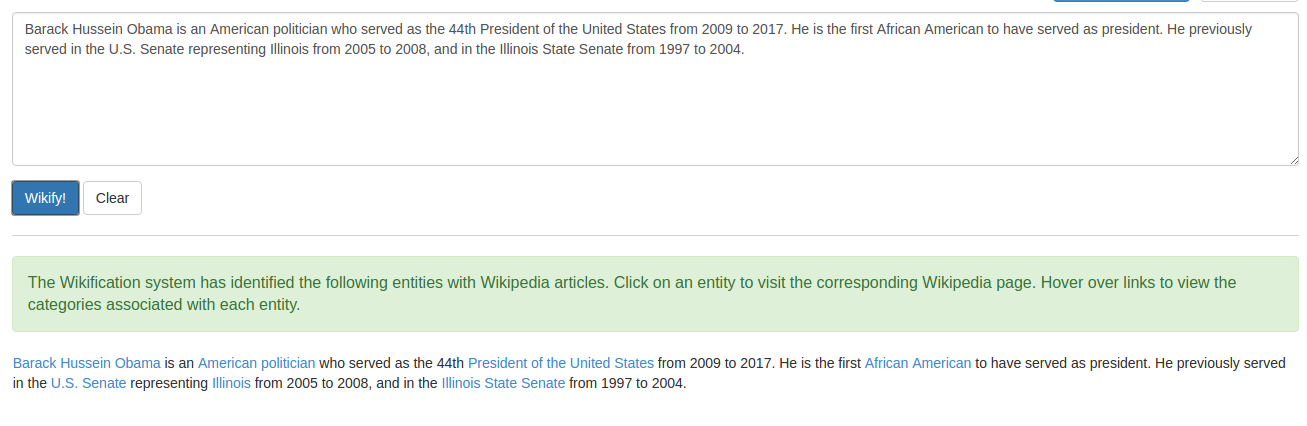
\includegraphics[scale=0.4]{images/eng.png}}
\captionof{figure}{Veličina entiteta skupa podataka na engleskom jeziku}

\end{center}

\begin{center}
  \makebox[\textwidth]{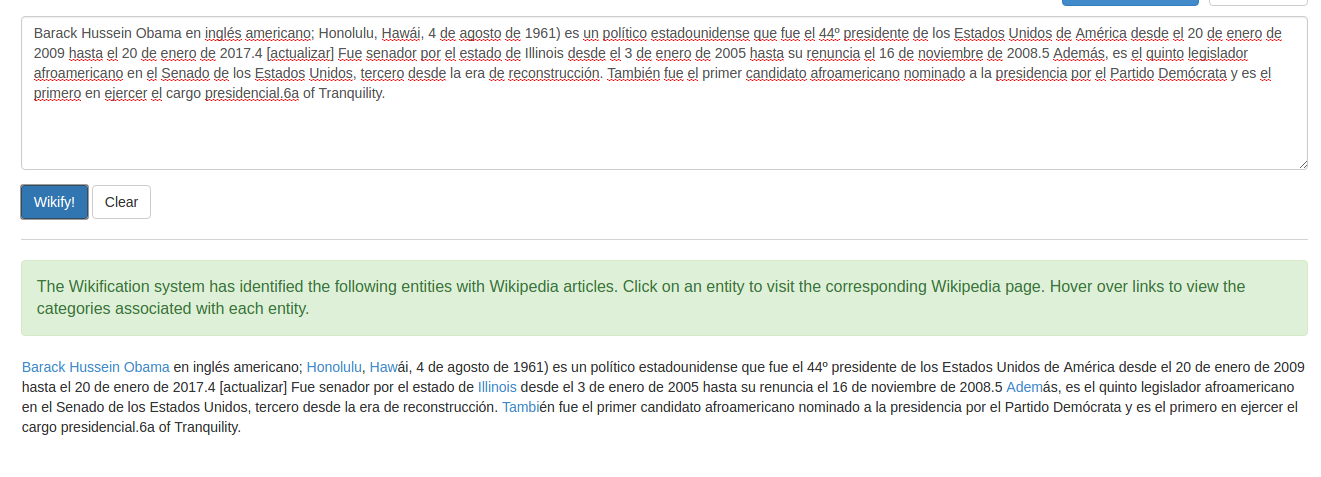
\includegraphics[scale=0.4]{images/esp.png}}
\captionof{figure}{Veličina entiteta skupa podataka na španjolskom jeziku}
\end{center}

\begin{center}
  \makebox[\textwidth]{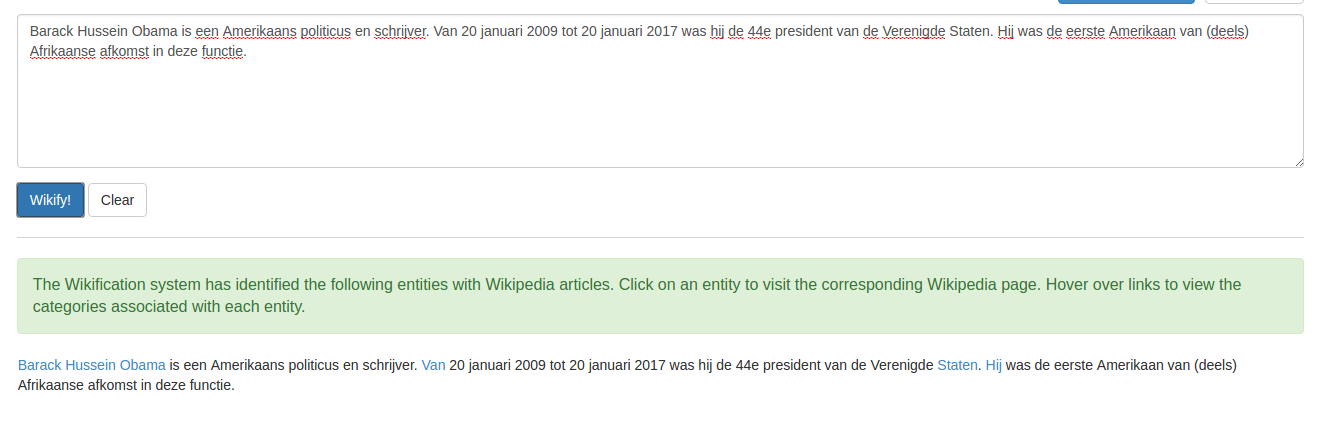
\includegraphics[scale=0.4]{images/ned.png}}
\captionof{figure}{Veličina entiteta skupa podataka na nizozemskom jeziku}
\end{center}
\chapter{Model}
U svrhu prepoznavanja imenovanih entiteta u tekstu najčešće se koriste sljedeći modeli: 
\begin{itemize}
\item HMM (Hidden Markov Model)
\item CRF (Conditional random field)
\item MaxEnt
\item Perceptron
\end{itemize}

Iako prva dva navedena modela daju mogućnost zajedničkog učenja oznaka u slijedu, ipak su korišteni Perceptron i MaxEnt modeli koji nam omogućuje korištenje raznih značajki.
\section{Perceptron}
\indent Perceptron je matematički model neurona. U stvarnom neuronu dendriti dobivaju signale od aksona drugih neurona dok su u matematičkom modelu dendriti predstavljeni s brojčanim vrijednostima. Izlaz neurona, akson, predstavljen je aktivacijskom funkcijom koja kao argument prima težinsku sumu ulaza neurona zbrojenom s pomakom.\footnote{\url{https://cs.stanford.edu/people/eroberts/courses/soco/projects/neural-networks/Neuron/index.htmls}}
\[ suma = \sum_{i=1}^{n} w_ix_i + b\]
\[ izlaz = activation\_function(suma) \]
\newpage
Perceptron pokušava naučiti težine na način da ih ne ažurira nakon prolaska kroz cijeli skup podataka već nakon svakog primjera. Ovakav način učenja se zove online učenje.  
\begin{center}
  \makebox[\textwidth]{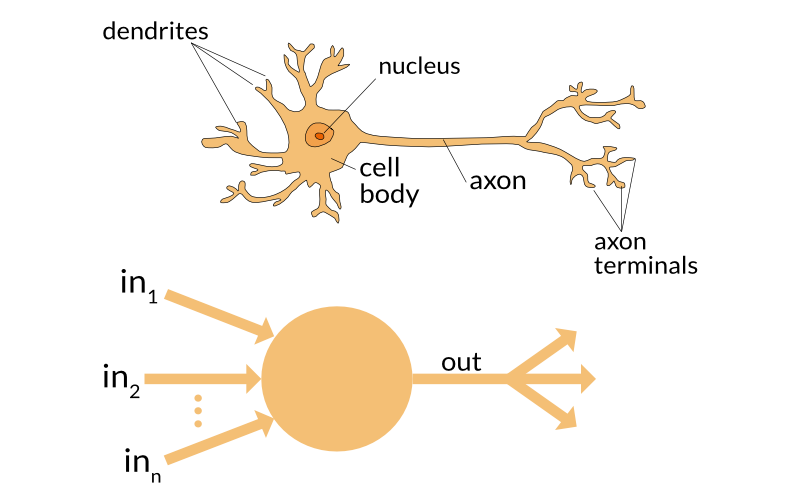
\includegraphics[scale=0.6]{images/neuron.png}}
\captionof{figure}{Matematički model biološkog neurona}\footnote{\url{https://appliedgo.net/perceptron/}}
\end{center}
\newpage
\section{Logistička regresija}
Logistička regresija je algoritam za binarnu klasifikaciju podataka. Treniranjem modela dobiva se vektor težina. Treniranje se obavlja korištenjem iterativnih algoritama kao sto je gradijentni spust.
Za predikciju klase kojoj primjer pripada koristi se logistička ili sigmoid funkcija.\footnote{\url{https://en.wikipedia.org/wiki/Sigmoid_function}} Kao argument te funkcije se dobiva skalarni produkt vektora značajki i vektora težina.\footnote{\url{http://ufldl.stanford.edu/tutorial/supervised/LogisticRegression/}}

\[ h_\theta(x) = \dfrac{1}{1+e^{-x}}\]

\begin{center}
  \makebox[\textwidth]{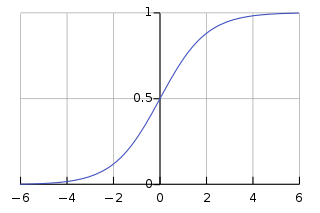
\includegraphics[]{images/log_fun.png}}
\captionof{figure}{Logistička ili sigmoid funkcija}\footnote{\url{https://upload.wikimedia.org/wikipedia/commons/thumb/8/88/Logistic-curve.svg/320px-Logistic-curve.svg.png}}
\end{center}

\chapter{Implementacija modela}
Sustav za prepoznavanje imenovanih entiteta je razvijen u programskom jeziku Python3. Korištena je implementacija Perceptrona\footnote{\url{http://scikit-learn.org/stable/modules/generated/sklearn.linear_model.Perceptron.html}} i Logističke regresije\footnote{\url{http://scikit-learn.org/stable/modules/generated/sklearn.linear_model.LogisticRegression.html}} iz scikit-learn knjižnice. U oba modela class\_weight parametar je postavljen na "balanced" što znači da model klase koje se rijetko pojavljuju unutar skupa za treniranje kažnjava više za grešku u predikciji jer sve klase smatra jednakima. Modeli su trenirani na 200 iteracija.
Glavni program runner.py pokreće cijeli cjevovod sustava. Moguće je specificirati jezike skupa za treniranje, validaciju i testiranje preko argumenata komandne linije. Naredba za pokretanje programa koji trenira i validira sustav engleskim i nizozemskim jezikom a testira nad španjolskim jezikom.
\begin{center}
python3 runner.py -train eng,ned -validation eng,ned -test esp
\end{center}

Nakon parsiranja argumenata dohvaćaju se navedeni skupovi za treniranje, validiranje i testiranje. Nakon toga se izvlače značajke iz podataka te se pretprocesiraju u brojčani oblik pogodan za algoritam. Prilikom odabira najboljeg modela radi se unakrsna validacija nad skupovima za treniranje i validiranje. 

Razvijena su tri modela koji se razlikuju u značajkama:
\begin{enumerate}
\item Osnovni model (engl. baseline) 
\item Osnovni model + Gazeteri
\item Osnovni model + Gazeteri + Wikifikacija
\end{enumerate}
\textbf{Gazeteri} su unaprijed prikupljeni skupovi entiteta. Za potrebe ovog modela prikupljeni gazeteri su podijeljeni u teme čiji su naslovi korišteni kao značajke modela. Neke od tema su: ArtWork, Building, Clothes, Films, Parks, Vehicles itd. Dodatno su prikupljeni skupovi za entitete Osoba, Organizacija i Lokacija te su za značajke korišteni kao broj pojavljivanja riječi u pojedinom skupu. Za dohvaćanja teme za neku riječ korišten je pomični prozor veličine $ 4 $. Ovisno o poziciji na kojoj se nalazi riječ u prozoru dodaje se prefiks B- ili I- temi kojoj pripada. Ako neka riječ ima više tema kojima pripada biramo prvu nađenu.\citep{DBLP:conf/conll/TsaiMR16} \\
Implementirani model za svaki token predviđa jednu od 9 klasa (O, B-PER, I-PER, B-ORG, I-ORG, B-LOC, I-LOC, B-MISC, I-MISC). Oznake B i I predstavljaju pocetak ili unutarnji dio entiteta prema BIO kodiranju imenovanih entiteta.\\\\
\textbf{Wikifikacija} je proces prepoznavanja entiteta u tekstu te povezivanja istih s nasličnijim stranicama na wikipediji. U referenciranom članku wikifikacija je iskorištena na način da se riječi i fraze iz tekstova koji nisu na engleskom jeziku mapiraju na stranice engleske wikipedije. Na taj način se dobivaju značajke koje nisu ovisne o jeziku na kojem je tekst pisan. Jedini uvjet je pristup stranicama Wikipedije na odabranom jeziku. U modelu razvijenom u članku wikifikacija je korištena tako da su prvo označili svaki 4-gram u tekstu. Nakon toga su svakoj riječi dali 3 značajke od kojih je svaka zapravo kategorija stranice na wikipediji i Freebase \footnote{\url{https://developers.google.com/freebase/guide/basic_concepts}} tip $ (w_{i-1}, w_{i}, w_{i+1}) $. \citep{DBLP:conf/conll/TsaiMR16}
\begin{center}
\captionof{table}{Broj gazetera za svaki entitet}
\begin{tabular}{ lcccc }
\hline
 & PER & LOC & ORG & MISC\\ 
\hline
Gazeteri & 2 972 k & 3 106 k & 977 k & 2 991 k \\
\hline
\end{tabular}
\end{center}

\newpage

\section{Značajke}
U tablici je naveden popis značajki podjeljen prema modelima u kojima su korištene.

\begin{center}
\captionof{table}{Značajke sustava}
\begin{tabular}{llr}
\hline
\textbf{Osnovne značajke} & \\
prethodni tag entiteta & $ (t_{i-1},t_{i-2}) $\\ 
sadrži samo brojke i slova & $ alphanumeric(w_i) $\\ 
sadrži samo brojke  & $ alldigits(w_i) $\\ 
sadrži samo veika slova & $ allcaps(w_i) $\\ 
sadrži samo brojke & $ iscapitalized(w_{i-2}, w_{i-1}, w_{i}, w_{i+1}, w_{i+2}) $\\
3-gram & suma pojavljivanja 3-grama za svaku klasu \\
\textbf{Gazeteri} & \\
naziv kategorije gazetera  & $ topic(w_{i}, w_{i+1}, w_{i+2}, w_{i+3}) $\\
broj pojavljivanja riječi u kategoriji & $ category\_count(w_{i}, \{PER, LOC, ORG\}) $\\
\textbf{Međujezične značajke} & \\
--- & ---\\

\hline
\end{tabular}
\end{center}

\section{Pretprocesiranje značajki}
Većina korištenih značajki su kategoričke stoga su kodirane Onehot \footnote{Svaka kategorija neke značajke se kodira u vektor duljine $ broj\_kategorija $ tako da je jedan element vektora $ 1 $ a ostali $ 0 $. \url{http://scikit-learn.org/stable/modules/generated/sklearn.preprocessing.OneHotEncoder.html}} metodom. Brojčane značajke kojima je definiran poredak skalirane su na interval $ [0,1] $. Za skaliranje je korišten MinMaxScaler\footnote{\url{http://scikit-learn.org/stable/modules/generated/sklearn.preprocessing.MinMaxScaler.html\#sklearn.preprocessing.MinMaxScaler}}.
\section{Unakrsna validacija}
Unaksrsna 5-struka validacija je korištena radi dobivanja najboljeg mogućeg modela za dane podatke. Parametri perceptrona koji su optimizirani unakrsnom validacijom: 

\[ alpha = (10^{-10}, 10^{-9}, ..., 10^{-2}) \]
\[ penalty = (l2, l1) \]

oba parametra se koriste u svrhu regularizacije,  alpha je konstanta koja množi regularizacijski faktor a penalty je regularizacijska funkcija.\\
Parametri logističke regresije korišteni za unakrsnu validaciju su:

\[ c = (10^{-7}, 10^{-9}, ..., 10^{2}) \]
\[ penalty = (l2, l1) \]
\chapter{Evaluacija}
Evaluacija sustava rađena je nad testnim skupom podataka. Model koji evaluiramo je najbolji model dobiven unakrsnom validacijom. Mjere koje su korištene za evaluaciju su f1-score, preciznost, odziv i točnost. Sustav je evaluiran na dva način:
\begin{enumerate}
\item Standardne mjere na razini svakog tokena.
\item Točno podudaranje gdje se entitet smatra dobro predviđenim ako se svaki token podudara po tipu s označenim podatcima.
\end{enumerate}

Ovisno o primjeni sustava u obzir se uzima jedna od dvije navedene metode evaluacije koja više odgovara primjeni. Metoda točnog podudaranja je dosta stroža od standardne evaluacijske metode. Prikazat ćemo način evaluacije na primjeru. Ako imamo sljedeću rečenicu u testnom skupu:\\\\
\centerline{[Leo]\textsubscript{B-PER} [Messi]\textsubscript{I-PER} played great match against [Real]\textsubscript{B-ORG} [Madrid]\textsubscript{I-ORG} in [Barcelona]\textsubscript{B-LOC}.}\\\\
a sustav je predvidio sljedeće oznake:\\\\
\centerline{[Leo]\textsubscript{B-PER} [Messi]\textsubscript{I-PER} played great match against [Real]\textsubscript{B-ORG} [Madrid]\textsubscript{B-LOC} in [Barcelona]\textsubscript{B-LOC}.}\\

Standardna točnost ove rečenice je 80\% dok se metodom točnog podudaranja dobije točnost 67\% jer cijeli entitet Real Madrid nije točan, dok se entitet Leo Messi broji kao jedan točan primjer.  

\begin{center}
\captionof{table}{Veličina skupova podataka}
\begin{tabular}{ lccc }
\hline
 & ENG & ESP & NED \\ 
\hline
Entiteti (treniranje) & 29 441 & 23 148 & 15 960 \\
Entiteti (testiranje) & 5 648 & 3 558 & 3 941 \\
\hline
\end{tabular}
\end{center}
\newpage
U sljedećim tablicama dane su f1-score mjere za jednojezične modele i međujezične modele trenirane na engleskom jeziku a testirane na drugima.

\begin{center}
\captionof{table}{Standardne evaluacijske mjere}
\begin{tabular}{ lcccc|cccc }
\hline
& \multicolumn{4}{c}{Perceptron} & \multicolumn{4}{c}{Log. regresija} \\ 
\cline{2-5}\cline{6-9}
 & ENG & ESP & NED & AVG & ENG & ESP & NED & AVG\\ 
\hline
\multicolumn{9}{c}{Jednojezični eksperimenti } \\
\hline
Osnovne značajke & 0.66 & 0.64 & 0.55 & 0.62 & 0.62 & 0.62 & 0.59 & 0.61 \\
+Gazeteri & 0.67 & 0.64 & 0.58 & 0.63 & 0.70 & 0.64 & 0.68 & 0.67 \\
+Wikifikacija & -- & -- & -- & -- & -- & -- & -- & -- \\
\hline
\multicolumn{9}{c}{Međujezični eksperimenti } \\
\hline
Osnovne značajke & -- & 0.59 & 0.56 & 0.575 & -- & 0.63 & 0.66 & 0.645 \\
+Gazeteri & -- & 0.61 & 0.54 & 0.575 & -- & 0.64 & 0.63 & 0. 635\\
+Wikifikacija & -- & -- & -- & -- & -- & -- & -- & -- \\
\hline
\end{tabular}
\end{center}


\begin{center}
\captionof{table}{Evaluacija metodom točnog podudaranja}
\begin{tabular}{ lcccc|cccc }
\hline
& \multicolumn{4}{c}{Perceptron} & \multicolumn{4}{c}{Log. regresija} \\ 
\cline{2-5}\cline{6-9}
 & ENG & ESP & NED & AVG & ENG & ESP & NED & AVG\\ 
\hline
\multicolumn{9}{c}{Jednojezični eksperimenti } \\
\hline
Osnovne značajke & 0.46 & 0.43 & 0.38 & 0.42 & 0.73 & 0.75 & 0.67 & 0.72 \\
+Gazeteri & 0.51 & 0.44 & 0.43 & 0.46 & 0.78 & 0.77 & 0.72 & 0.76 \\
+Wikifikacija & -- & -- & -- & -- & -- & -- & -- & --  \\
\hline
\multicolumn{9}{c}{Međujezični eksperimenti } \\
\hline
Osnovne značajke & -- & 0.29 & 0.31 & 0.30 & -- & 0.46 & 0.47 & 0.465 \\
+Gazeteri & -- & 0.33 & 0.28 & 0.305 & -- & 0.44 & 0.41 & 0.425 \\
+Wikifikacija & -- & -- & -- & -- & -- & -- & -- & --  \\
\hline
\end{tabular}
\end{center}
\newpage
U sljedećem grafu prikazane su f1 mjere modela treniranog na jezicima na y-osi, a testiranog na jezicima na x-osi. Crvena boja označava bolju mjeru. Ako treniramo model na engleskom jeziku a testirano na nizozemskom dobivamo f1 score 0.5.

\begin{center}
  \makebox[\textwidth]{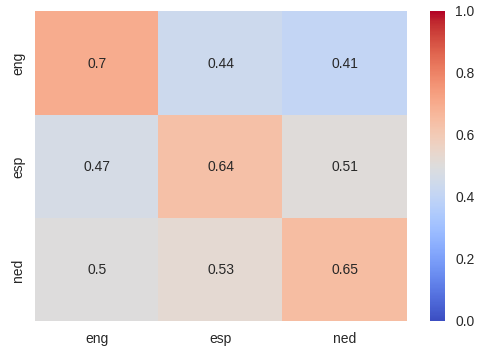
\includegraphics[]{images/corr_plot.png}}
\captionof{figure}{Evaluacijska matrica modela s različitim jezicima za treniranje i testiranje. Korištena je f1 mjera. Evaluacija je iyvršena na modela koji uključuje baseline i gazetere.}
\end{center}

\section{Poboljšanja}
Poboljšanja se kriju u boljoj kvaliteti podataka i otkrivanju nekih bolji značajki. Konkretno za razvijeni model u ovom radu pri odluci koji tema gazettera će biti dodjeljena trenutno promatranoj riječi dobije se pronalaskom te riječi u skupu teme. Poboljšanje možemo ostvariti presjekom tema s okolnim riječima jer ne pripada neka riječ samo jednoj temi. Uključivanje word embeddinga kao značajke za svaku riječ bi moglo rezultirati poboljšanjem. Metoda Wikifikacije se može poboljšati boljom distribucijom kategorija i obogaćivanjem wikipedije za jezike s manjim resursima.
\chapter{Zaključak}
Potreba za komunikacijom i razumijevanjem svih jezika je veća nego ikad uslijed naglog razvoja interneta i mogućnosti povezivanja ljudi iz raznih dijelova svijeta. Također, dijeljenje znanja je lakše nego ikad. Većina zapisa na internetu je na engleskom jeziku stoga za engleski jezik postoje najbolji modeli za analizu jezika. Prepoznavanje imenovanih entiteta u tekstu je zadataka primjenjiv u raznim područjima. Za jezike s malo resursa nemamo dovoljno dobre modele za prepoznavanje. Zbog toga posežemo za malo drugačijim pristupom. Želimo iskoristiti dobre modele na engleskom jeziku za poboljšanje modela resursno siromašnijih jezika.\\
\indent U ovom radu je razvijen model po uzoru na \citep{DBLP:conf/conll/TsaiMR16} gdje je iskorištena wikifikacija za povezivanje entiteta na wikipedijama različitih jezika. Nažalost, zbog nemogućnosti iskorištavanja već gotovih programa za wikifikaciju te zbog nedostatka vremena i težine zadatka razvijanja vlastitog modela wikifikacija nije korištena te međujezični model nije davao dobre rezultate. Zbog toga razvijeni model radi puno bolje na jednojezičnim postavkama. Iako je hrvatska Wikipedija siromašna, zanimljivo bi bilo primjeniti ovaj pristup na hrvatskom jeziku.\\
\indent Prostora za poboljšanje modela ima još puno kako u ovom  tako i korištenjem nekih drugačijim pristupa.

\bibliographystyle{fer}
\bibliography{literatura}
\nocite{*}

\begin{sazetak}

Zbog stalnog rasta svih vrsta podataka, naročito teksta ljudi više nisu u mogućnosti obraditi te podatke da bi prepoznali bitne i korisne informacije. Zbog toga posežemo za računalnom obradom podataka. U ovom radu razvijen je model za međujezično prepoznavanje imenovanih entiteta. Za razvoj dobrog modela za klasifikaciju potrebno nam je puno podataka. Prema zadnjim procjenama više od $ 50\% $ sadžaja na internetu je pisano na engleskom jeziku. Motivacija za razvoj međujezičnog modela leži u potpunoj dominaciji engleskog jezika u svim vrstama podataka i NLP alata. Razvojem takvog modela jezici sa skromnim izvorima podataka bi napredovali ne samo u prepoznavanju imenovanih entiteta već u analizi teksta općenito.

\kljucnerijeci{Strojno učenje, Procesiranje prirodnog jezika, Prepoznavanje imenovanih entiteta, Perceptron}
\end{sazetak}
% TODO: Navedite naslov na engleskom jeziku.
\engtitle{Cross-Lingual Named Entity Recognition via Wikification}
\begin{abstract}
Because of the steady growth of all kinds of data, especially text, people are no longer able to process this data to recognize essential and useful information. That's why we reach for computer data processing. In this paper, a model for cross-lingual named entity recognition was developed. To develop a good model for classification we need a lot of data. According to the latest estimates, more than $ 50 \% $ of web content is written in English. Motivation for the development of an cross-lingual model lies in the overall dominance of English in all types of data and NLP tools. By developing such a model, languages with modest data sources would advance not only in the recognition of named entities, but in text analysis in general.


\keywords{Machine learning, Natural language processing, Named entity recognition, Perceptron}
\end{abstract}

\end{document}
